\documentclass[12pt]{article}\usepackage[]{graphicx}\usepackage[dvipsnames]{xcolor}
% maxwidth is the original width if it is less than linewidth
% otherwise use linewidth (to make sure the graphics do not exceed the margin)
\makeatletter
\def\maxwidth{ %
  \ifdim\Gin@nat@width>\linewidth
    \linewidth
  \else
    \Gin@nat@width
  \fi
}
\makeatother

\definecolor{fgcolor}{rgb}{0.345, 0.345, 0.345}
\newcommand{\hlnum}[1]{\textcolor[rgb]{0.686,0.059,0.569}{#1}}%
\newcommand{\hlstr}[1]{\textcolor[rgb]{0.192,0.494,0.8}{#1}}%
\newcommand{\hlcom}[1]{\textcolor[rgb]{0.678,0.584,0.686}{\textit{#1}}}%
\newcommand{\hlopt}[1]{\textcolor[rgb]{0,0,0}{#1}}%
\newcommand{\hlstd}[1]{\textcolor[rgb]{0.345,0.345,0.345}{#1}}%
\newcommand{\hlkwa}[1]{\textcolor[rgb]{0.161,0.373,0.58}{\textbf{#1}}}%
\newcommand{\hlkwb}[1]{\textcolor[rgb]{0.69,0.353,0.396}{#1}}%
\newcommand{\hlkwc}[1]{\textcolor[rgb]{0.333,0.667,0.333}{#1}}%
\newcommand{\hlkwd}[1]{\textcolor[rgb]{0.737,0.353,0.396}{\textbf{#1}}}%
\let\hlipl\hlkwb

\usepackage{framed}
\makeatletter
\newenvironment{kframe}{%
 \def\at@end@of@kframe{}%
 \ifinner\ifhmode%
  \def\at@end@of@kframe{\end{minipage}}%
  \begin{minipage}{\columnwidth}%
 \fi\fi%
 \def\FrameCommand##1{\hskip\@totalleftmargin \hskip-\fboxsep
 \colorbox{shadecolor}{##1}\hskip-\fboxsep
     % There is no \\@totalrightmargin, so:
     \hskip-\linewidth \hskip-\@totalleftmargin \hskip\columnwidth}%
 \MakeFramed {\advance\hsize-\width
   \@totalleftmargin\z@ \linewidth\hsize
   \@setminipage}}%
 {\par\unskip\endMakeFramed%
 \at@end@of@kframe}
\makeatother

\definecolor{shadecolor}{rgb}{.97, .97, .97}
\definecolor{messagecolor}{rgb}{0, 0, 0}
\definecolor{warningcolor}{rgb}{1, 0, 1}
\definecolor{errorcolor}{rgb}{1, 0, 0}
\newenvironment{knitrout}{}{} % an empty environment to be redefined in TeX

%\usepackage{alltt}
\usepackage{amsmath,amsfonts,amssymb,graphicx,authblk}
\usepackage[font={footnotesize,singlespacing},labelfont=bf]{caption}
\usepackage{titlesec,blkarray, bm} 
\usepackage{float,afterpage}
\usepackage[running,mathlines]{lineno}
\usepackage[vmargin=1in,hmargin=1in]{geometry}
\usepackage[authoryear,sort]{natbib}
\usepackage[dvipsnames]{xcolor}
\usepackage[nodisplayskipstretch]{setspace} 
\usepackage[section]{placeins}
\usepackage{gensymb}
\usepackage{enumitem}
\usepackage{orcidlink}
\usepackage{tabularx} % put this once in your preamble
\usepackage{booktabs}
\usepackage{pdflscape}  % or \usepackage{lscape}
\usepackage{adjustbox}
\usepackage{newfloat}   % for creating new float types
\usepackage{tocloft}    % for customizing lists
\usepackage{caption}
\usepackage{rotating}
\usepackage{xr-hyper} % cross-references between main text and SI
\usepackage{hyperref}
\externaldocument{../Supplementary_LaTeX/EcolLett_R2_SI}
\usepackage{makecell} % 
\usepackage{longtable}
\usepackage{pdflscape}
\setlist{topsep=.125em,itemsep=-0.15em,leftmargin=0.75cm}
\setlength{\parindent}{0.35in}

\usepackage[sc]{mathpazo} %Like Palatino with extensive math support
\usepackage[subtle]{savetrees}

\usepackage{lineno}
%\renewcommand{\refname}{Literature Cited}
%\renewcommand{\floatpagefraction}{0.9}
%\renewcommand{\topfraction}{0.99}
%\renewcommand{\textfraction}{0.05}

\clubpenalty = 10000
\widowpenalty = 10000

\sloppy 

\usepackage{ifpdf}
\ifpdf
\DeclareGraphicsExtensions{.pdf,.png,.jpg}
\DeclareFloatingEnvironment[fileext=losf, listname={List of Supplementary Figures}]{suppfigure}
\DeclareFloatingEnvironment[fileext=lost, listname={List of Supplementary Tables}]{supptable}
\usepackage{epstopdf}
\else
\DeclareGraphicsExtensions{.eps}
\fi

%\graphicspath{{/Users/jacobmoutouama/Dropbox/Miller Lab/github/endo-range-limits/Manuscript/Ecology letters/Manuscript/LaTexR1/Figure}}
%\graphicspath{{C:/Users/tm9/Dropbox/github/ELVI-endophyte-density/Figure}}
\newcommand{\tom}[2]{{\color{red}{#1}}\footnote{\textit{\color{red}{#2}}}}
\newcommand{\jacob}[2]{{\color{blue}{#1}}\footnote{\textit{\color{blue}{#2}}}}
\renewcommand\Authfont{\normalfont\normalsize}    % sets author names to small
\renewcommand\Affilfont{\normalfont\small} % sets affiliations even smaller
\newcommand{\revise}[1]{{\color{Mahogany}{#1}}}
%\newcommand{\Sminus}{S\revise{\textminus{}}}
%\renewcommand{\thesuppfigure}{S\arabic{suppfigure}}
%\renewcommand{\thesupptable}{S\arabic{supptable}}
\setlength{\affilsep}{1em}  
%\doublespacing



% I cannot get \orcidlink working on my computer so for now replacing this with \textit

%-------------------------------------------------------------------------
\title{\Large Aridity and herbivory shape demographic benefits of fungal endophytes in cool-season grasses}
\author[1, 2]{Jacob K. Moutouama\,\orcidlink{0000-0003-1599-1671} \thanks{Corresponding author: jmoutouama@gmail.com}}
\author[3]{Joshua C. Fowler}
\author[4]{Akiem M. Gough}
\author[4]{Julia Martin}
\author[4]{Christopher C. Oxley}
\author[4]{Karl M. Schrader}
\author[4]{Karis Williams}
\author[4]{Tom E.X. Miller\,\orcidlink{0000-0003-3208-6067}}
\affil[1]{Department of Botany, University of British Columbia, Vancouver, BC, Canada}
\affil[2]{African Centre for DNA Barcoding, University of Johannesburg, Johannesburg, South Africa}
\affil[3]{Department of Environmental Studies, University of Colorado Boulder, Boulder, CO, USA}
\affil[4]{Department of BioSciences, Rice University, Houston, TX, USA}
\date{} % clear date


\sloppy

%-------------------------------------------------------------------------
\IfFileExists{upquote.sty}{\usepackage{upquote}}{}
\frenchspacing
\begin{document}
%\SweaveOpts{concordance=TRUE}
\renewcommand{\baselinestretch}{1.2}
\maketitle
\vspace{-2.5em}
% \bigskip 
%45 character limit on running head
\noindent\textbf{Running Title:} Stress and Grass-Endophyte Symbioses\\
\noindent\textbf{Keywords:} demography, mutualism, plant--fungi interactions, range limits, stress gradient hypothesis, symbiosis\\
\bigskip 
\noindent\textbf{Article Type:} Letter

\bigskip 
\noindent\textbf{Data accessibility statement:} 
All data and analysis scripts supporting the results are archived on Zenodo ([DOI link]).

\bigskip 
\noindent\textbf{Conflict of interest statement:} None.

\bigskip
\noindent\textbf{Acknowledgments}
This research was supported by National Science Foundation Division of Environmental Biology award 2208857. We gratefully acknowledge the individuals and institutions who hosted our geographically-distributed experiment, including the University of Louisiana, Sam Houston State University, Texas A\&M University, and University of Texas at Austin. 
JKM was supported by start-up research funds GR036071 from the University of British Columbia and by NSERC grants GR038661 and GR038746. 
JCF was supported by an NSF Postdoctoral Fellowship in Biology (DBI 2410282).
Three anonymous reviewers provided constructive feedback on an earlier version of this paper.


\bigskip
\noindent\textbf{Authorship statement:} J.K.M. contributed to research conception, data collection, data analysis, and led manuscript drafting and revision.
J.C.F., J.M., A.M.G., C.C.O., K.M.S., and K.W. contributed to data collection and manuscript revisions. T.E.X.M. contributed to research conception, data collection, data analysis, and manuscript revisions.


\bigskip
\noindent\textbf{This file contains:} Abstract (150 words), Main Text (4998 words), Figures (1-6), References (73). Supporting Information is provided as a separate file.

\newpage
%\SweaveOpts{concordance=TRUE}
\linenumbers
%-------------------------------------------------------------------------
\spacing{1.25}
\section*{Abstract}
Plant–microbe symbioses are expected to enhance host resilience to environmental stress, yet whether symbiont effects differ across abiotic versus biotic stress dimensions remains unclear. 
We tested how aridity and herbivory shape fitness effects of vertically transmitted fungal endophytes on three grass host species using herbivore exclusion experiments along a precipitation gradient in the south-central United States. 
Contrary to predictions, endophyte-associated hosts showed stronger declines in demographic performance with aridity than endophyte-free plants, suggesting abiotic stress exacerbated symbiont costs. 
Endophyte symbiosis reduced herbivory for two host species, consistent with protective benefits, but herbivore exclusion effects were weaker and more idiosyncratic relative to climate stress. 
A greenhouse experiment using soils from field sites showed endophyte effects were not strongly sensitive to soil origin, supporting a causal role of climate in driving site-level variation. 
Together, these results challenge the expectation that stress enhances symbiosis benefits and suggest limited buffering potential under increasing aridity.
\bigskip

%--------------------------------------------------------------------
\newpage
\section*{Introduction}
Mutualistic symbioses are widespread and ecologically important, often mediating stress tolerance and defense against natural enemies for host organisms. 
Host--symbiont interactions, like mutualisms more broadly, are strongly context-dependent, with outcomes shaped by environment \citep{hoeksema2015context, bronstein1994conditional,hoang2024impacts,rudgers2020climate}. 
The stress-gradient hypothesis (SGH) is a classic conceptual framework for variation in interaction outcomes, predicting that the frequency of positive interactions increases under stressful conditions \citep{louthan2015and,bertness1994positive,holmgren2010strong,maestre2009refining}.
%, but actual outcomes depend on the type and intensity of biotic and abiotic stress
For example, microbial symbionts that are costly to maintain under benign conditions may benefit host plants under drought stress  \citep{giauque2019endophyte}. 
Stress can take many forms, including abiotic and biotic factors, and it remains unclear how predictions of the SGH for host--symbiont interactions play out over different dimensions of environmental stress. 
%Variation in the nature and intensity of biotic and abiotic stress is thus a key driver of these context-dependent outcomes. 
%As symbiotic interactions shift along stress gradients, their effects are predicted to become increasingly beneficial under biotic and abiotic stress, enhancing host resilience to stress.

Under biotic stress, such as competition or attack by natural enemies, symbionts can mediate defensive traits across diverse taxa \citep{atala2022fungal,bastias2017epichloe,vega2008insect,haine2008symbiont,florez2015defensive}.
Similarly, under abiotic stress, including drought, nutrient limitation, and thermal extremes, symbiotic partners often enhance host tolerance through improved resource acquisition, physiological regulation, and stress-responsive metabolism \citep{clay2002evolutionary, afkhami2008symbiosis,cesar2024defensive}. 
In plants specifically, microbial symbionts such as mycorrhizal fungi, rhizobia, and endophytic bacteria and fungi can promote water and nutrient uptake, nitrogen fixation, and resistance to herbivores, allowing hosts to maintain growth and function under harsh abiotic or biotic conditions \citep{amijee1989development, friesen2011microbially,van2015mycorrhizal}.
Many plant symbionts also stimulate the production of antioxidant enzymes, reducing oxidative damage caused by stressors such as drought, salinity, and heat \citep{ruiz1996superoxide}. 
By improving resource acquisition, modulating physiology, and enhancing stress-responsive metabolism, these interactions help host plants buffer against environmental extremes \citep{fowler2023geographic,rudgers2020climate,li2026climate}.

%Although microbial symbioses often enhance plant performance, they can also impose substantial costs, particularly in resource-limited environments. 
Environmental stress can shift the balance of costs and benefits between hosts and their symbiotic microbes, and the direction and magnitude of this shift can depend on stress severity and environmental context.
In plants, maintaining symbionts requires hosts to allocate valuable carbon and nutrients to their microbial partners; for example, mycorrhizal fungi can demand up to 20\% of a host's photosynthetically fixed carbon \citep{thirkell2020carbon,soudzilovskaia2015quantitative}.
Under stress, this investment can outweigh benefits, reducing survival, growth, or reproduction \citep{johnson1997functioning,bronstein2001exploitation,klironomos2003variation}.
A parallel dynamic occurs in coral bleaching, where heat stress can disrupt the coral--algal mutualism, with thermal thresholds for breakdown relatively well quantified compared with those in most other symbioses \citep{evensen2022empirically,vidal2009coral,marangon2025destabilization}. Across systems, symbiotic microbes can therefore either mitigate or exacerbate host responses to environmental stress, depending on stress severity, the type and combination of stressors, and characteristics of the interacting partners \citep{david2018microbial,michalet2007highlighting,kawai2007testing,le2010interaction}. Thus, although the classic SGH predicts that positive interactions should strengthen with increasing stress, extensions of the hypothesis recognize that positive interactions can weaken or become neutral or antagonistic under sufficiently severe stress.
However, the environmental and biological conditions under which the balance shifts from beneficial to neutral or detrimental remain poorly understood. Identifying these conditions is essential for predicting when stress will strengthen mutualistic outcomes and when it will instead impose demographic costs on hosts.

Despite growing interest in symbiosis and host demography under environmental stress, few studies have tested how abiotic and biotic stressors synergistically shape the costs and benefits of symbiosis to host organisms.
In a greenhouse study of \emph{Ammophila breviligulata}, symbiont-associated plants grew more than symbiont-free plants under either herbivory or drought alone, but this benefit disappeared when the two stressors were combined, with symbiont-associated and symbiont-free plants showing similar growth \citep{emery2010variation}.
Studying the combined effects of abiotic and biotic stressors under natural conditions is particularly important in the context of global change \citep{louthan2015and}, as shifting climate patterns and altered herbivore pressures may change the balance of costs and benefits in plant–microbe interactions, potentially influencing species distributions and ecosystem function \citep{reynolds2003grassroots}.
Understanding how abiotic stress, biotic stress, and microbial symbiosis interact requires experiments that manipulate all three factors simultaneously, yet such fully factorial studies remain rare outside controlled settings.
Here, we address this gap by examining the demographic effects of endophyte symbiosis on three grass host species spanning a natural range-core/range-edge precipitation gradient and in the presence/absence of herbivores.
%providing insight into how these biotic and abiotic stressors influence endophyte prevalence, host fitness component such as survival, growth and reproduction under realistic environmental conditions.

Symbioses between cool-season grasses and seed-transmitted fungal endophytes (\textit{Epichloë} spp.) provide a powerful experimental model for studying how abiotic and biotic elements of ecological context influence host–symbiont interactions \citep{schardl2004symbioses,saikkonen2010defensive,oberhofer2014effects,clay2005herbivores}. 
Because vertical transmission links host and symbiont fitness, it is expected to favor the evolution of mutualistic interactions \citep{gundel2024temporal,gundel2011incorporating}. 
Environmental conditions, including long-term variation in precipitation, temperature, and herbivore exposure, strongly influence both the prevalence of \textit{Epichloë} infection and the benefits conferred to hosts \citep{clay2005herbivores,rudgers2016long,fowler2025increasing}. 
For example, grasses hosting \textit{Epichloë} endophytes often outperform endophyte-free individuals under water limitation, though the magnitude of these benefits depends on both host and symbiont identity \citep{decunta2021systematic}. 
A key benefit of \textit{Epichloë} symbiosis is the production of fungal alkaloids that deter herbivores or reduce herbivore performance, thereby mediating plant–herbivore interactions \citep{saikkonen2010defensive,crawford2010fungal}.
Fungal alkaloids may also modify host osmotic balance in ways that promote water use efficiency \citep{decunta2021systematic}. 
Endophytes may impose costs on their hosts, including the carbon resources required to sustain the fungus and reduced growth or reproduction when fungal demands exceed host resource supply \citep{bennett2022costs}. 
Finally, \textit{Epichloë} endophyte effects can differ in both magnitude and direction among host vital rates, such that symbiosis may benefit one vital rate while having neutral or negative effects on another. 
For example, symbiosis may not improve survival under stress but can still enhance growth or reproduction \citep{yule2013costs,rudgers2012there}.
 
We established experimental gardens of three species of native cool-season grasses with and without fungal endophytes across an aridity gradient in the south-central United States to investigate how symbiosis affects multiple host vital rates under varying abiotic and biotic stress. 
At each of seven sites along the aridity gradient, we manipulated vertebrate and invertebrate herbivory (allowing herbivore access versus exclusion) to test its interaction with abiotic stress.
We asked whether endophyte symbiosis is beneficial for host grasses, whether benefits are amplified under abiotic and/or biotic stress as predicted by the stress-gradient hypothesis (SGH), and how these stressors interact to shape demographic outcomes. 
We evaluated four alternative hypotheses (Fig.~\ref{fig:prediction}):
\begin{enumerate}
\item Context-independent mutualism: Endophytes confer consistent positive effects on host demography across environmental conditions (Fig.~\ref{fig:prediction}a).
\item Herbivory-dependent effects: Endophyte benefits are greater under herbivore exposure than under herbivore exclusion, independent of the abiotic environment, consistent with a defensive role of fungal alkaloids (Fig.~\ref{fig:prediction}b).
\item Climate-dependent effects: Endophyte benefits decline with increasing precipitation, such that symbiont effects are more positive under arid than wet conditions, independent of herbivore exposure (Fig.~\ref{fig:prediction}c).
\item Herbivory- and climate-dependent effects: The effect of endophyte symbiosis depends on the joint influence of herbivory and precipitation, such that exposure to herbivory amplifies endophyte benefits under more arid conditions (Fig.~\ref{fig:prediction}d).
\end{enumerate}
Finally, to supplement the geographically-distributed field experiment and isolate the causal role of climatic factors, we used a greenhouse experiment with one host species to assess the influence of edaphic factors that co-vary with precipitation across experimental sites. 

%--------------------------------------------------------------------
\section*{Materials and methods}
\subsection*{Study system}
Our study focused on three cool-season perennial grass species native to woodland, savanna, and grassland habitats of eastern North America: \emph{Agrostis hyemalis}, \emph{Elymus virginicus}, and \emph{Poa autumnalis} (Poaceae, subfamily Pooideae) \citep{shaw2011guide}.
\revise{\linelabel{spab1}\emph{Agrostis hyemalis}} is a short-lived perennial that germinates from autumn to late winter and, in our Texas study region, typically flowers between April and June.
\revise{\linelabel{spab2}\emph{Elymus virginicus}} is a larger, longer-lived species that flowers throughout spring and summer.
\revise{\linelabel{spab3}\emph{Poa autumnalis}} has a similar growth form to \emph{E. virginicus} and flowers in late spring.
\revise{\linelabel{spab4}\emph{Agrostis hyemalis}} hosts the endophyte \emph{Epichloë amarillans} \citep{white1994endophyte}, \emph{Elymus virginicus} hosts \emph{Epichloë elymi} \citep{liu2023fungi}, and \emph{Poa autumnalis} hosts \emph{Epichloë} PauTG-1 or \emph{E. poae} \citep{gundel2020simulated}.
Previous studies of these associations have generally found beneficial effects on host performance, although effects can vary among host species, vital rates, and environmental conditions \citep{yule2013costs,davitt2011understanding,gundel2020simulated,rudgers2009benefits}.
Like other \emph{Epichloë} species, these endophytes are primarily transmitted vertically through seeds but some are additionally capable of horizontal transmission via sexual stromata on inflorescences or asexual conidia on leaf surfaces \citep{clay2002evolutionary,gundel2020simulated,leuchtmann2014nomenclatural}.
In our study, stromata were never observed on \emph{E. virginicus} or \emph{P. autumnalis} and were rarely observed on \emph{A. hyemalis} ($<5\%$ of individuals), suggesting a dominant role of vertical transmission.
Herbivory in this system is primarily from deer, generalist insects (aphids, grasshoppers), and small mammalian grazers.

\subsection*{Source populations and symbiont removal}
Plants used in our experiment were derived from 11 natural source populations located throughout the ranges of the focal species (Fig.~\ref{fig:site}, Table~\ref{tab:source_pop}). 
Seeds from these source populations (collected from ca. 30 individuals per population) were either heat-treated to remove endophytes or left untreated (control), intended to produce lineages of symbiont-free ($S^-$) and symbiotic ($S^+$) plants from the same genetic background. 
For \emph{E. virginicus} and \emph{P. autumnalis}, heat-treated seeds were placed in a drying oven at 60°C for five days. 
For \emph{A. hyemalis}, seeds were heat-treated in a water bath at 60°C for 12 min.
For all but two populations, the $S^-$\ plants used in our experiment were reared through one or more generations following heat treatment, which minimized the confounding potential of direct physiological effects of heating seeds (Table \ref{tab:heat_treatment}). 
Seeds from control and heat-treated lineages were surface-sterilized with a  10\% bleach solution \citep{Sahu2022sterilization}.

Seedlings were transferred to potting soil and maintained in the Rice University greenhouse at 18--29~$^\circ$C and ambient photoperiod.
Once plants were sufficiently large, they were vegetatively propagated to generate the required sample sizes, with clonal identities tracked across individuals. 
We refer to each independently derived source individual (originating from a single seed) as a ``genotype'' and consider all of its vegetatively propagated descendants to belong to the same genotype, such that all clones share the same genetic background of the host and (for $S^+$) symbiont.
The experiment included 840, 840, and 720 plants of \textit{A. hyemalis}, \textit{E. virginicus}, and \textit{P. autumnalis}, respectively, with half assigned to each endophyte status ($S^+$ and $S^-$), from three, four, and four source populations, respectively.
The breakdown of these aggregate totals among source populations, genotypes, and clonal replicates per genotype is reported in Table~\ref{tab:source_pop}.
Endophyte status of all genotypes was verified prior to field transplant using microscopy and immunoblot assays (see Supplementary Methods).


\subsection*{Common garden experimental design and climate data}
We established common garden experiments with $S^+$ and $S^-$ hosts at seven sites along an aridity gradient from Louisiana to central Texas, US (Fig.~\ref{fig:site}, Table~\ref{tab:exp_sites}).
From west to east, mean annual precipitation increases more than three-fold across these sites while mean annual temperature is relatively consistent, based on climate data collected during the same period as our demographic surveys (Fig.~\ref{fig:site}d, Fig. \ref{sup:temp}).
For this reason, we focus on precipitation as the primary abiotic factor that varied across sites.  
This geographic gradient overlaps and exceeds the natural range edges of our focal species, ensuring exposure to realistic climatic and biotic conditions (Fig.~\ref{fig:site}a, b, c). 

To characterize climate at these sites during the study period (2023–2025), we collected monthly temperature and precipitation data from PRISM at 800 m resolution \citep{PRISM2024}. 
For each site, we calculated mean temperature (\textdegree C) and cumulative precipitation (mm) over each demographic interval, from the census month in year $t$ through the census month in year $t+1$.

At each of seven sites along the gradient, we established 24 plots (1.5 m $\times$ 1.5 m), eight per host species (\textit{P. autumnalis} was planted at six sites, excluding the westernmost site (SON) since it is well outside this species' natural range: Fig.~\ref{fig:site}c).
Each plot was planted with 15 individuals, with 12, 9, 6, or 3 $S^+$ plants and the remainder $S^-$, corresponding to initial endophyte frequencies of 80\%, 60\%, 40\%, or 20\% $S^+$, respectively.
 \revise{\linelabel{spacing}Plants were arranged in an evenly spaced 4 $\times$ 4 grid, approximately 37.5~cm apart, with the 16th grid position left unplanted.}
This variation in initial endophyte prevalence was intended to track change in prevalence from different starting conditions and is not further considered here.
Within each site, each plot was randomly assigned to either herbivore access or herbivore exclusion (Fig.~\ref{fig:site}e).
The herbivory treatment targeted both vertebrate and invertebrate herbivores: exclusion plots had deer fencing on four sides and were sprayed with Sevin insecticide (active ingredient zeta-cypermethrin) 2--3 times per growing season following the manufacturer's protocol; herbivore access plots were unsprayed and fenced on two sides to control for any fence effect.

Greenhouse-raised plants were planted into the field experiment in February--March 2023.
For each species at each site, we planted a total of 60 $S^+$ and 60 $S^-$ plants, half of those experiencing herbivore access and half experiencing herbivore exclusion. 
Clonal replicates were arranged such that all plots had the same genetic diversity (number of genotypes) for each species. 
%Initial endophyte prevalence varied from 20\% (3 $S^+$, 12 $S^-$) to 80\% (12 $S^+$, 3 $S^-$); this aspect of the experimental design was intended to address a different question about change in symbiont prevalence across generations, and is not further considered here. 
Plots at the two westernmost sites (KER and SON) were destroyed by deer soon after planting in 2023 and subsequently replanted in 2024 with stronger fencing.
Because demographic responses were calculated between consecutive censuses, observations from replanted plots were treated as new $t$--$t+1$ demographic intervals. We also repeated the analyses excluding KER and SON to assess whether the disturbance and subsequent replanting influenced our results.


\subsection*{Demographic data collection}
We collected demographic data, including survival, growth, and reproduction, during the flowering season of each species in 2023, 2024, and 2025: \emph{Agrostis hyemalis} and \emph{Poa autumnalis} were censused in May, and \emph{Elymus virginicus} in June.
For each individual, survival was recorded as alive or dead and, for surviving plants, size was measured as the number of tillers.
For surviving plants, growth was quantified as the log ratio of tiller count between consecutive censuses (i.e., $\log(\text{tiller}_{t+1}/\text{tiller}_{t})$).
We recorded the number of inflorescences per plant for all species and, for reproducing individuals of \emph{Poa autumnalis} and \emph{Elymus virginicus}, counted spikelets on a maximum of three inflorescences per plant. Spikelet counts were not recorded for \emph{Agrostis hyemalis} because its inflorescences contain numerous, very small spikelets that are difficult to count reliably in the field.
%\revise{\linelabel{spikeletmethod}Spikelets were counted on up to three inflorescences per plant.}
%In \emph{A. hyemalis}, one spikelet yields one seed, \revise{\linelabel{whereas1}whereas} in \emph{P. autumnalis} and \emph{E. virginicus}, a single spikelet can produce 2--6 seeds.
%Spikelet counts were limited to three reproducing tillers per plot due to the time-consuming nature of this measurement.  

We measured herbivore damage to assess the effects of symbiont status and herbivore exclusion treatment on realized herbivory. 
For each individual at each census, we counted the number of tillers with any signs of herbivory (leaf chewing or clipped tillers) and quantified the proportion of total tillers with herbivore damage. 
We also binned plants as damaged/undamaged based on the presence/absence of any damaged tillers, and tallied the proportion of damaged plants by plot, site, and herbivore treatment.

\subsection*{Statistical modeling}
To assess how abiotic and biotic stress modify the demographic effects of endophyte symbiosis, we fit generalized linear mixed models for each vital rate response in a hierarchical Bayesian statistical framework. %first developed two candidate models for each vital rate: one quadratic and one monotonic.
All models shared the same hierarchical structure for their expected values and were applied to survival, growth, and fertility (inflorescence count and, for two species, spikelet count per inflorescence).
Survival was modeled with a Bernoulli distribution, growth with a Gaussian distribution, inflorescence count with a negative binomial hurdle model, and spikelet count with a negative binomial distribution. 
Hurdle and zero-inflated negative binomial models had nearly identical predictive performance ($\Delta$ELPD = 0.2, SE = 3.1).
We retained the hurdle model because it distinguishes whether a plant flowered and, if so, how many inflorescences it produced. Its two components, a Bernoulli model for flowering and a zero-truncated negative binomial model for inflorescence count, both used the linear predictor in Eq.~\ref{eq:full_model}.

All models included species-specific fixed effects for symbiosis ($S^+$ or $S^-$), site- and year-specific precipitation, and herbivory (herbivore access/exclusion), as well as all two- and three-way interactions among them.
Quadratic effects of precipitation did not improve predictive performance over linear effects (LOOCV; Table~\ref{tab:model_comparison}), so we used the linear model, in which the expected value for observation $i$ ($\mu_{i}$) was:
%Each observation $i$ corresponds to a plant in a given year; individuals can appear in multiple years. 
%For simplicity, we omit the full subscript notation for species, plot, population, and site-year, which is explicitly included in the Stan model. 
\begin{equation}\label{eq:full_model}
\begin{aligned}
\mu_i &= \beta_0[Sp_i] + \beta_P[Sp_i] * precip_i + \beta_{E}[Sp_i]\, * symb_i + \beta_{H}[Sp_i]\, * herb_i \\
&\quad + \beta_{EP}[Sp_i]\, * symb_i * precip_i 
       %+ \beta_{symb \times P^2}[Sp_i]\, symb_i P_i^2 
       + \beta_{HP}[Sp_i]\, * herb_i * precip_i \\
&\quad + \beta_{HE}[Sp_i]\, * herb_i * symb_i + \beta_{HEP}[Sp_i]\, *symb_i * herb_i * precip_i \\
&\quad  + \phi_{\text{site}[i],Sp_i} 
       + \omega_{\text{source}[i]} 
       + \rho_{\text{plot}[i]}
       \\
&\quad \quad \quad \quad \phi_{\text{site}[i],Sp_i} \sim N(0,\ \sigma^2_{site})\\
&\quad \quad \quad \quad \rho_{\text{plot}[i]} \sim N(0,\ \sigma^2_{plot})\\
&\quad \quad \quad \quad \omega_{\text{source}[i]} \sim N(0,\ \sigma^2_{source})
\end{aligned}
\end{equation}
Here, $\mathrm{precip}_i$ is the natural logarithm of cumulative precipitation (mm) over the demographic interval, standardized to mean zero and unit variance; $\mathrm{symb}_i$ indicates endophyte presence ($\mathrm{symb}_i = 1$) or absence ($\mathrm{symb}_i = 0$), and $\mathrm{herb}_i$ indicates fencing treatment: herbivore access ($\mathrm{herb}_i = 0$) or exclusion ($\mathrm{herb}_i = 1$).
The model includes random effects accounting for background variation at multiple hierarchical levels: $\phi_{\text{site}[i],Sp_i}$ captures site-to-site heterogeneity that is not explained by precipitation, $\rho_{\text{plot}[i]}$ captures plot-to-plot variation within sites, and $\omega_{\text{source}[i]}$ captures variation associated with the provenance of transplants (the latter two are unique to species and therefore not indexed by species).
Random effects for site, plot, and source are host species-specific but the variance parameters ($\sigma_{\text{site}}$, $\sigma_{\text{source}}$, $\sigma_{\text{plot}}$) are shared across species; this assumes, for example, that site-to-site heterogeneity is of a similar magnitude across species, even as the model allows for ``better'' and ``worse'' sites to differ by species. 
This hierarchical structure allows the model to ``borrow strength'' across species \citep{gelman2007data}, improving estimates of fixed effects while still capturing species-specific responses to the environmental gradient.

Models were implemented in R \citep{RCoreTeam} using Stan via \texttt{rstan} \citep{Rstan}, with four chains of 3,000 iterations (1,000 warm-up), weakly informative normal priors on fixed effects, and diffuse priors on random-effect variances (full details in the accompanying code). 
Posterior predictive checks confirmed adequate model fit (Fig.~\ref{sup:ppc_vital}).

We used posterior probability distributions of the parameter estimates to visualize predictions for how effects of symbiosis varied across abiotic and biotic contexts.
For each herbivory treatment (Access or Exclusion), we computed posterior predictions for the vital rates of $S^+$ and $S^-$ hosts across the precipitation gradient (Eq.~\ref{eq:full_model}).
From these predictions, we calculated the difference for each posterior sample ($\Delta = \mu^{+} - \mu^{-}$) to estimate mean effects and 90\% credible intervals.
We then computed the posterior probability that $\Delta > 0$, which quantifies the probability that endophytes enhance performance, given the model and data.
For instance, a high posterior probability (e.g., Pr$(\Delta>0) >0.9$) indicates strong evidence of an endophyte benefit, whereas a low posterior probability (e.g., Pr$(\Delta>0) <0.1$) indicates strong evidence of an endophyte cost.
Intermediate probabilities (approximately 0.7--0.9 or 0.1--0.3) indicate moderate evidence for positive or negative effects, respectively, whereas probabilities near 0.5 indicate no evidence for a directional effect.


\subsection*{Greenhouse experiment}
We used site variation to capture an aridity gradient, but other abiotic factors, especially edaphic conditions, covary across sites. 
In particular, the two westernmost sites (KER and SON; Fig. \ref{fig:site}) are not only the driest but also occur on the Edwards Plateau of central Texas, with distinct limestone soils.
If edaphic variation rather than precipitation drives the symbiont $\times$ precipitation interaction observed in the field, we would expect the interaction to persist in the greenhouse, where soils from contrasting sites are brought into a common climate. 
Conversely, if the field pattern reflects a genuine climate-mediated effect of the symbiosis, the interaction should disappear when plants are decoupled from the climate of their soil's origin. 
To distinguish between these alternatives, we conducted a greenhouse experiment using \textit{A. hyemalis} and soils collected from each field site, crossing symbiont status ($S^+$/$S^-$) with soil origin (seven sites; Fig.~\ref{fig:site}d; 
Table~\ref{tab:soil_pop}; Supplementary Methods~\ref{sec:greenhouse}).
Using data on biomass and inflorescence production in the greenhouse, we fitted similar hierarchical Bayesian models as the field analysis, with symbiont status, soil-origin precipitation (30-year normal, standardised), and their interaction as fixed effects (Supplementary Methods~\ref{sec:greenhouse_models}).
Posterior predictive checks showed good agreement between the observed data and data simulated from the posterior distributions, indicating that the models adequately captured the main features of the observed biomass and inflorescence production data (Fig.~\ref{sup:ppc_models_soil}).

\section*{Results}
\subsection*{Efficacy of aridity and herbivory treatments}
%\revise{\linelabel{herbivoryefficacity}
%As intended, realized precipitation and herbivory treatments tracked the abiotic and biotic gradients targeted by our design. 
%Realized precipitation at the seven experimental sites corresponded well to 30-year climate normals, with wetter eastern sites and drier western sites (Fig.~\ref{fig:site}d). 
%Herbivore exclusion also decreased realized herbivory: plants in herbivore-access plots experienced 24\% tiller damage on average, compared to 14\% in herbivore-exclusion plots (Fig.~\ref{sup:herb}; Fig.~\ref{sup:herbsp}; Fig.~\ref{sup:herbivory}).
%}
As intended, realized precipitation and herbivory treatments tracked the abiotic and biotic gradients targeted by our design. 
Realized precipitation at the seven experimental sites corresponded well to 30-year climate normals, with wetter eastern sites and drier western sites (Fig.~\ref{fig:site}d). 
Herbivore access also increased realized herbivory: plants in herbivore-access plots experienced 24\% tiller damage on average, compared to 14\% in herbivore-exclusion plots (Fig.~\ref{fig:site}f; Fig.~\ref{sup:herb}; Fig.~\ref{sup:herbsp}; Fig.~\ref{sup:herbivory}).
Endophyte symbiosis reduced the predicted proportion of damaged tillers in \textit{P. autumnalis} ($S^+$: 13.5\% vs.\ $S^-$: 17.1\%) and, more weakly, in \textit{A. hyemalis} ($S^+$: 12.8\% vs.\ $S^-$: 14.2\%), whereas it increased damage in \textit{E. virginicus} ($S^+$: 62.8\% vs.\ $S^-$: 59.4\%; Fig.~\ref{sup:herbivory}).

\subsection*{Endophyte effects on host fitness components across abiotic and biotic stress gradients}
Annual survival was greater overall and more positively responsive to precipitation for the longer-lived hosts \textit{E. virginicus} and \textit{P. autumnalis} compared to the shorter-lived \textit{A. hyemalis} (Fig.~\ref{fig:Surv}; Fig.~\ref{sup:coef_caterpillar}).
Endophyte effects on survival depended most strongly on precipitation in \textit{E. virginicus}. 
Under herbivore exclusion, effects of endophytes on survival shifted from strongly negative under dry conditions ($\Delta = -0.13$, $\mathrm{Pr}(\Delta > 0) = 0.02$) to positive under wetter conditions ($\Delta = 0.12$, $\mathrm{Pr}(\Delta > 0) = 0.97$; Table~\ref{tab:delta_summary_surv_quantiles}). 
Under herbivore access the same directional shift occurred but with weaker magnitude ($\Delta = -0.06$ to $0.10$, $\mathrm{Pr}(\Delta > 0) = 0.10$--$0.89$). 
A similar but weaker directional shift occurred in \textit{A. hyemalis} under both herbivory treatments.
For the host \textit{P. autumnalis}, survival was strongly responsive to climate variation but there was no evidence that symbionts modified the response to climate stress, and there was little difference between herbivory treatments (Fig.~\ref{fig:allstat}, Fig.~\ref{fig:Surv}).

For growth, endophyte benefits increased with precipitation in \textit{A. hyemalis} and \textit{E. virginicus} under herbivore access, with strong positive effects of symbiosis under the wettest conditions (\textit{A. hyemalis}: $\Delta = 0.49$, $\mathrm{Pr}(\Delta > 0) = 0.99$; \textit{E. virginicus}: $\Delta = 0.32$, $\mathrm{Pr}(\Delta > 0) = 0.97$; Fig.~\ref{fig:growth}; Table~\ref{tab:delta_summary_grow}). 
Under herbivore exclusion, \textit{A. hyemalis} showed a similar positive trend but with weaker support ($\Delta = 0.29$, $\mathrm{Pr}(\Delta > 0) = 0.90$), while \textit{E. virginicus} showed little variation across the gradient ($\Delta = 0.09$--$0.10$, $\mathrm{Pr}(\Delta > 0) = 0.60$--$0.75$). 
For both \textit{A. hyemalis} and \textit{E. virginicus}, endophyte effects on growth were most beneficial under wetter abiotic conditions and herbivore access (Fig.~\ref{fig:growth}a--d). 
As for survival, \textit{P. autumnalis} growth rates declined strongly under drier conditions but endophyte effects were weak and highly uncertain (Fig.~\ref{fig:allstat}). 
Under herbivore exclusion, endophyte effects on \textit{P. autumnalis} growth shifted from weakly positive to negative with increasing precipitation ($\Delta = -0.22$, $\mathrm{Pr}(\Delta > 0) = 0.13$), the only species–vital rate combination that was even directionally consistent with drought-protective benefits of symbiosis.

For inflorescence production, endophyte effects were strongly positive in \textit{P. autumnalis} and increased with precipitation under both herbivory treatments (Fig.~\ref{sup:inflo}; Table~\ref{tab:delta_summary_flow}). 
Under herbivore access, effects ranged from weak under drier conditions ($\Delta = 0.02$, $\mathrm{Pr}(\Delta > 0) = 0.68$) to strongly positive under wetter conditions ($\Delta = 2.91$, $\mathrm{Pr}(\Delta > 0) = 0.99$). 
Under herbivore exclusion, benefits were consistently strong across the gradient ($\Delta = 0.19$--$4.97$, $\mathrm{Pr}(\Delta > 0) = 0.97$--$1$). 
In contrast, endophyte effects on inflorescence production were weaker and highly uncertain across the gradient in the hosts \textit{A. hyemalis} and \textit{E. virginicus} under both herbivory treatments (Fig.~\ref{sup:inflo}; Fig.~\ref{fig:allstat}). 
Spikelet production in \textit{E. virginicus} and \textit{P. autumnalis} was climate-sensitive; endophyte effects on spikelets increased with precipitation under herbivore exclusion but were weak under herbivore access (Fig.~\ref{sup:spikelet}; Fig.~\ref{sup:spike_delta}; Table~\ref{tab:delta_summary_spike}).


%, endophyte effects were generally weak under herbivore access in both \textit{A. hyemalis} ($\Delta = -2.33$ to $0.74$, $\mathrm{Pr}(\Delta > 0) = 0.23$--$0.62$) and \textit{E. virginicus} ($\Delta = -0.76$ to $0.84$, $\mathrm{Pr}(\Delta > 0) = 0.35$--$0.67$). 
%Under herbivore exclusion, however, effects shifted from negative at dry sites to positive at wet sites in \textit{A. hyemalis} ($\Delta = 3.20$, $\mathrm{Pr}(\Delta > 0) = 0.94$) and were consistently positive across the gradient in \textit{E. virginicus} ($\Delta = 2.73$--$3.46$, $\mathrm{Pr}(\Delta > 0) = 0.81$--$0.98$; Fig.~\ref{sup:spikelet}).

Figure \ref{fig:allstat} synthesizes statistical confidence in endophyte effects across host species, vital rates, and abiotic and biotic stress gradients. 
The broad trend that emerged was a shift from negative or neutral endophyte effects under drier conditions to more positive effects under wetter conditions.
These patterns were largely consistent with the hypothesis that abiotic (climate) stress is the dominant modifier of endophyte effects (Hypothesis 3; Fig.~\ref{fig:prediction}c), but in the opposite direction from that predicted, as endophyte benefits tended to increase rather than decrease with precipitation. 
Partial support emerged for herbivory and combined effects of herbivory and climate as symbiosis modifiers (Hypotheses 2 and 4; Fig.~\ref{fig:prediction}b,d), depending on species and fitness component. 
Herbivory played a secondary role for most species and vital rates. 
Herbivore exclusion generally dampened the growth benefits that hosts gained from endophytes, consistent with an anti-herbivore protective role of \textit{Epichloë} endophytes. 
However, the role of herbivory as a modifier of endophyte effects on  other vital rates was more idiosyncratic. 

Plots at the two westernmost sites (KER and SON) were destroyed by deer and replanted in 2024.
We therefore repeated all analyses excluding these sites to assess whether their replanting influenced our conclusions.
Excluding KER and SON produced qualitatively similar patterns of symbiont effects across climate and herbivory treatments (Fig.~\ref{fig:sensitivity_KER_SON}, Table~\ref{tab:sensitivity_KER_SON}), indicating that our conclusions were not driven by the replanted sites.

 \subsection*{Greenhouse experiment: soil legacy effects do not mediate endophyte responses}
In the greenhouse experiment with \textit{A. hyemalis} growing on soils from each experimental site, fitness components responded strongly to soil origin even under uniform conditions: plants grown in soils from wetter sites produced greater aboveground biomass and more inflorescences than those from drier-origin soils (Figs.~\ref{fig:biomass_inflo}a--b), confirming that soil properties co-vary with the field precipitation gradient. However, the estimated symbiont effects on both aboveground biomass and inflorescence production showed little systematic variation with soil-origin precipitation (Fig.~\ref{sup:greenhouse_coef}; Table~\ref{tab:posterior_soil}). Thus, although soil origin affected plant performance, it did not explain the variation in symbiont effects associated with precipitation in the field.

\section*{Discussion}
Drawing on three years of field experiments and Bayesian analysis of host demography, we evaluated how biotic and abiotic stressors jointly influence the demographic effects of vertically transmitted \textit{Epichloë} endophytes on three cool-season perennial grasses across a natural climatic gradient. We predicted that endophytes would enhance host fitness under aridity and/or herbivore pressure (Fig.~\ref{fig:prediction}), in line with stress amelioration and defense scenarios.
Our results are inconsistent with context-independent mutualism (Fig.~\ref{fig:prediction}a): endophyte effects varied substantially across host species and along the precipitation gradient rather than remaining constant.
They are also inconsistent with the climate-dependent hypothesis as formulated (Fig.~\ref{fig:prediction}c), which predicted more positive endophyte effects under arid than wet conditions; instead, benefits were strongest under benign, mesic conditions and weakened as abiotic stress increased, the opposite of the predicted direction.
Support for the herbivory-dependent hypothesis (Fig.~\ref{fig:prediction}b) was mixed: effects of herbivore exclusion on endophyte benefits were inconsistent across species and fitness components, although the strongest effects were in the predicted direction, with herbivore exclusion dampening endophyte benefits for growth.
We found little evidence for the herbivory--climate-dependent hypothesis (Fig.~\ref{fig:prediction}d), as herbivory did not consistently amplify endophyte benefits under more arid conditions.
More broadly, the benefits of symbiosis depended on stress severity and host performance: they were greatest when symbiont-free hosts performed relatively well, but diminished or turned negative when those hosts performed poorly. 
This pattern is consistent with extensions of the SGH in which positive interactions weaken or shift toward antagonism under sufficiently severe stress \citep{le2010interaction,kawai2007testing,michalet2007highlighting}.

The physiological mechanisms underlying the decline in endophyte benefits with increasing aridity are unclear, but several non-exclusive processes may contribute.
Reduced water availability may limit the host's capacity to benefit from the symbiosis through constrained nutrient uptake, reduced carbon gain, or drought-induced hormonal shifts that impair endophyte function or alter the cost--benefit balance of the interaction \citep{ahlholm2002vertically, bronstein2001exploitation, faeth2002endophytic, bastias2024epichloe, cui2022abscisic}.
This interpretation aligns with the microbial mitigation--exacerbation continuum \citep{david2018microbial}, which predicts that symbionts can shift from beneficial to costly as environmental stress exceeds the host's capacity to sustain the interaction. 
Our results are also consistent with empirical patterns along precipitation gradients in other grass--\textit{Epichloë} systems \citep{rudgers2009benefits}, and by a systematic review noting that positive endophyte effects on drought tolerance are inconsistent across species and understudied for fitness measures such as fecundity and survival \citep{decunta2021systematic}.

\revise{\linelabel{ms-loss}Endophyte loss under drought may also contribute to the decline in endophyte benefits with increasing aridity.}
\revise{Endophyte infections are not always maintained throughout the host life cycle, and environmental conditions can influence their persistence \citep{afkhami2008symbiosis,david2019testing}.}
\revise{If endophyte loss occurred at the drier sites of our gradient, some plants hosting the symbiont at the start of the experiment may have lost their endophyte, potentially weakening the measured differences between symbiotic and non-symbiotic plants.}
We did not track endophyte status throughout the experiment and therefore cannot test this possibility directly. The likelihood and consequences of endophyte loss may depend on host--symbiont specialization and functional differences among endophytes \citep{saona2010environmental}. Future studies should track endophyte status over time and assess host resource status across aridity gradients and host--endophyte systems to determine how these factors contribute to variation in the demographic benefits of symbiosis.

Host species differed in how strongly increasing aridity altered the demographic benefits of \textit{Epichloë}.
  \revise{\linelabel{spab5}\textit{Poa autumnalis}} maintained strong reproductive benefits across the climatic gradient, whereas effects on survival and growth were weaker.
In contrast, \textit{A. hyemalis} and \textit{E. virginicus} showed 
more pronounced climate-dependent responses in survival and growth, suggesting that these vital rates may be more responsive to climatic variation near their arid range margins.
These contrasts may reflect differences in host physiological tolerance, symbiont identity, or the ecological contexts in which each species evolved \citep{decunta2021systematic}, and highlight the importance of considering multiple vital rates when evaluating grass--endophyte symbioses under climate stress \citep{cheplick2009ecology}.

Herbivore exclusion generally dampened endophyte benefits for growth across species, consistent with an anti-herbivore protective role of \textit{Epichloë} endophytes reinforced under natural herbivore pressure \citep{clay1988fungal, decunta2021systematic}. 
Effects of herbivory on survival and reproduction were more idiosyncratic, varying across species and precipitation contexts, suggesting these consequences are not uniformly mediated by herbivore pressure across fitness components. 
Endophytes reduced herbivore damage in \textit{A. hyemalis} and \textit{P. autumnalis}, in keeping with alkaloid-mediated defense, but increased damage in \textit{E. virginicus} (Fig.~\ref{sup:herbivory}), possibly because symbiotic plants were more vigorous and therefore more attractive to herbivores.
These species-specific responses may reflect differences in alkaloid identity and potency among endophytes \citep{siegel1990fungal}, together with host condition. 
Thus, the effects of endophytes on herbivory may depend on both the defensive chemistry of the symbiont and the condition of the host.

The greenhouse experiment suggests that the symbiont--climate interaction observed in the field is more closely linked to the direct physiological effects of water availability on the host than to soil properties that co-vary with aridity. 
Although soil origin affected plant performance under common watering conditions, the negligible symbiont $\times$ soil-origin precipitation interactions for biomass and inflorescence production indicate that this soil gradient did not reproduce the climate dependence of symbiont effects observed in the field. 
Thus, soil properties can influence host performance, but are unlikely to be the primary driver of climatic variation in symbiont benefits. Instead, direct effects of water availability on host carbon balance, growth, and resource allocation may influence the strength of the association. 

The precipitation gradient spanned by our common gardens overlaps with the range margins of the grass species we studied, making our findings relevant to host persistence near range margins. \revise{\linelabel{range-expansion}Although endophytes can alleviate drought stress and potentially influence host distributions, their effects on host performance are context-dependent \citep{afkhami2014mutualist}. In our study, endophyte-associated hosts showed stronger declines in demographic performance with increasing aridity, suggesting that endophytes do not necessarily buffer hosts against abiotic stress. These demographic responses may not translate directly into changes in population growth or geographic range, neither of which we directly estimated. Whether endophytes promote host persistence or range expansion under increasing aridity, and how climate-driven changes in endophyte prevalence influence these outcomes, remain open questions \citep{fowler2025increasing,li2026climate}.}
Future work should distinguish climate-driven changes in endophyte persistence from changes in their effects on host performance, as these mechanisms may have different consequences for host populations at range margins.
\newpage
%\bibliographystyle{plain}
\bibliographystyle{apalike}
\bibliography{References}

\clearpage
\section*{Figures}

\captionsetup[figure]{list=no}
\begin{figure}[htbp]
\centering
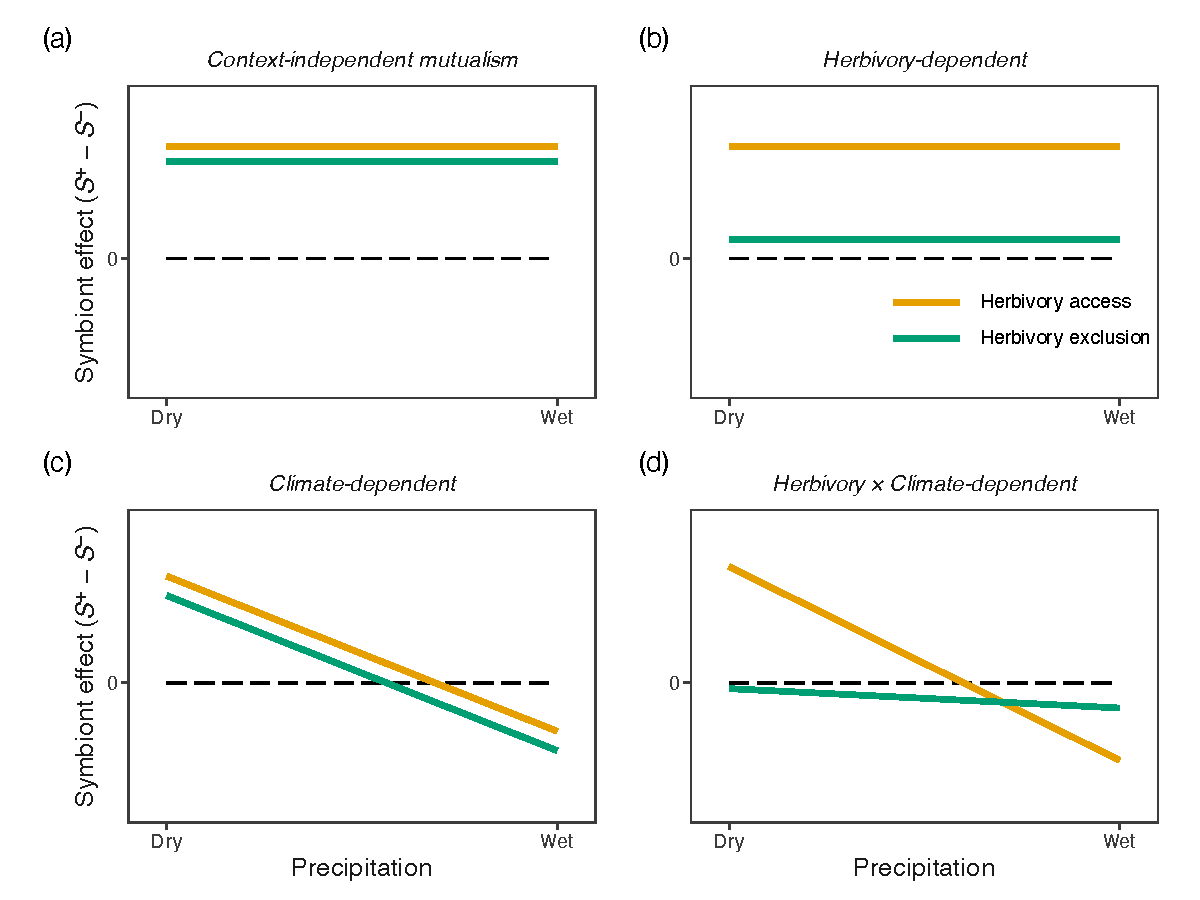
\includegraphics[width=1\textwidth]{conceptual_figure.pdf}
\caption{
Competing hypotheses for how plant–symbiont interactions vary along a precipitation gradient under contrasting herbivory regimes. Positive values for the demographic contrast of $S^+ - S^-$ indicate beneficial effects, and negative values indicate costly effects of symbionts. (a) Context-independent mutualism, where symbiont effects remain constant across environmental conditions and herbivory treatments. (b) Herbivory-dependent interactions, where the effect of symbionts differs in magnitude between herbivore access and exclusion but is insensitive to climate. (c) Climate-dependent interactions, where symbiont effects shift systematically along the precipitation gradient, independent of herbivory. (d) Combined herbivory- and climate-dependent interactions, where both environmental context and biotic pressure jointly shape symbiont effects, resulting in non-parallel and potentially decoupled response trajectories. Together, these scenarios illustrate alternative hypotheses for how symbiotic interaction outcomes may vary across abiotic and biotic stress gradients.
}
\label{fig:prediction}
\end{figure}
\clearpage

\captionsetup[figure]{list=no}
\begin{figure}[htbp]
\centering
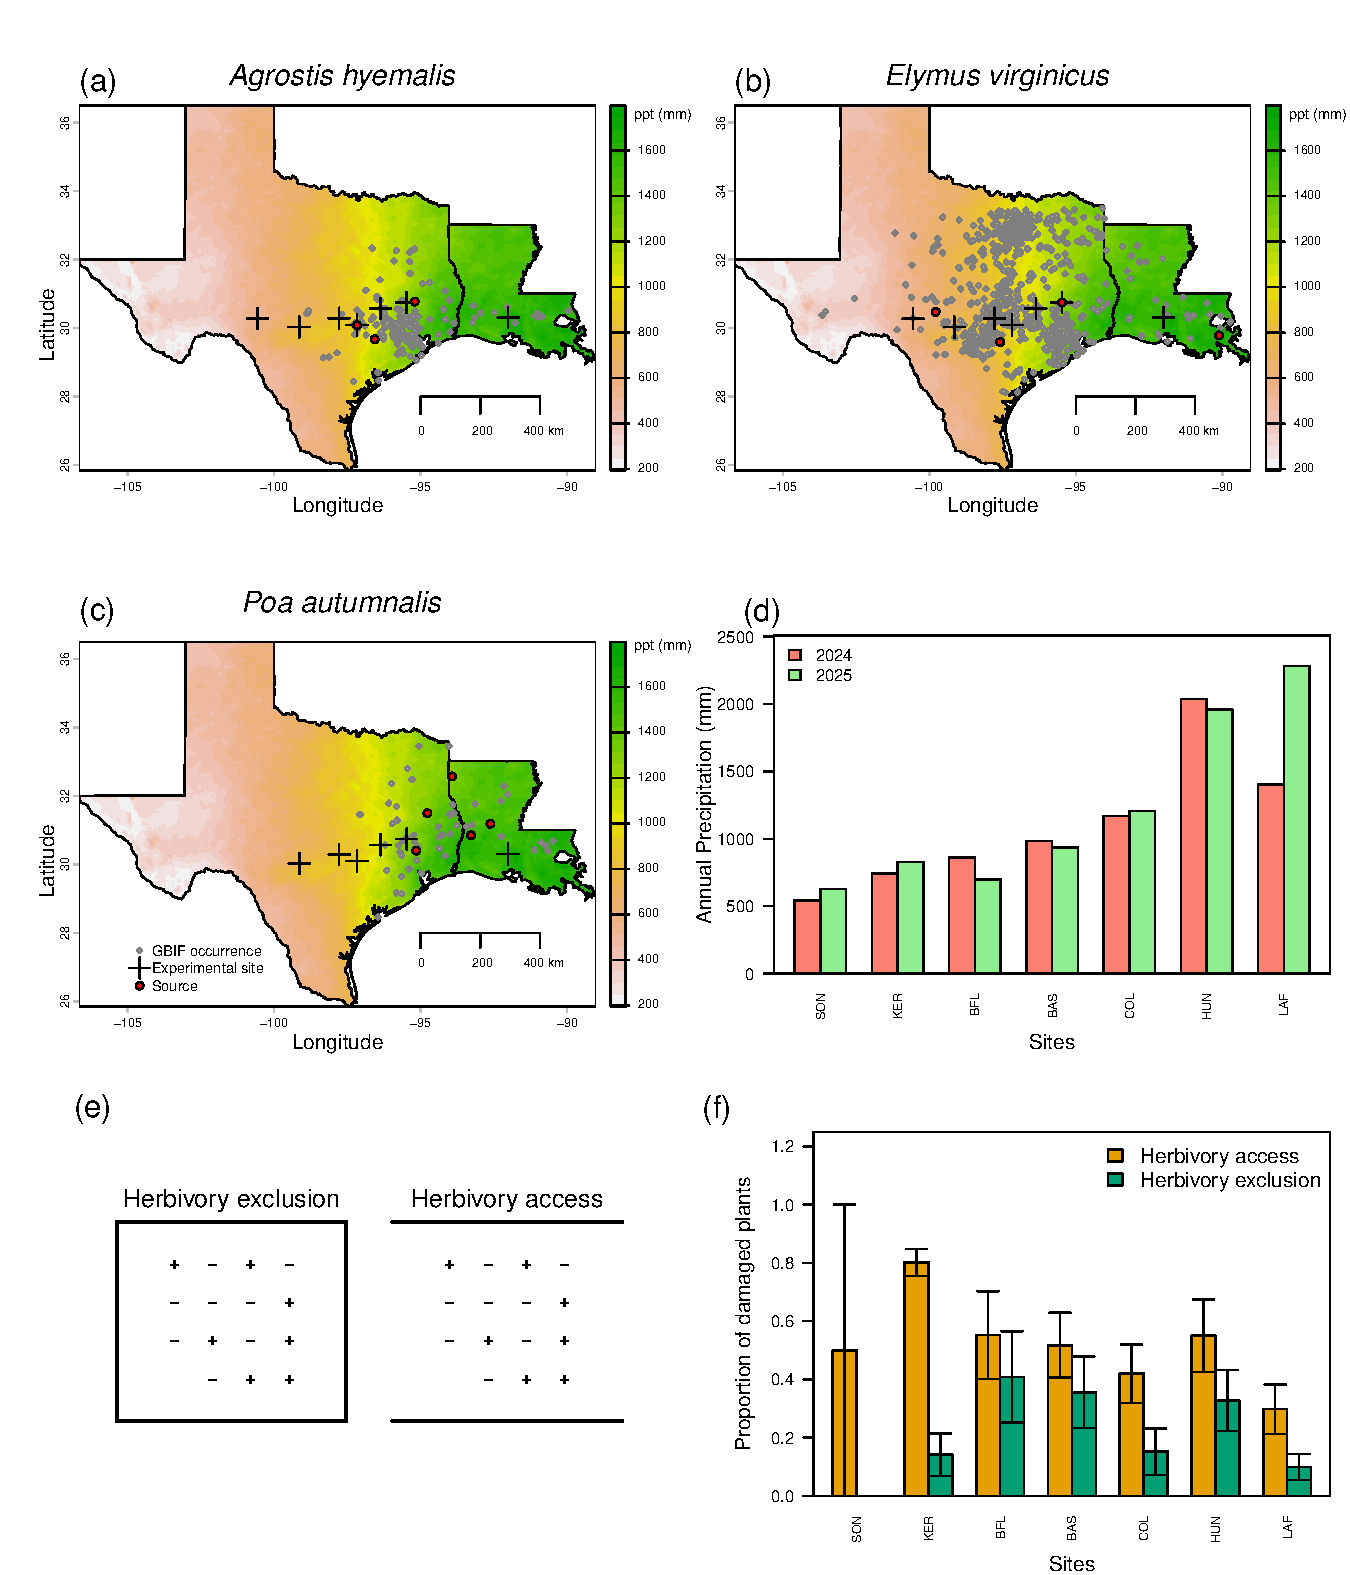
\includegraphics[width=0.92\textwidth]{clim_map1.pdf}
\caption{Geography of common garden sites along a natural aridity gradient from Texas to Louisiana, USA for (a) \emph{Agrostis hyemalis}, (b) \emph{Elymus virginicus}, and (c) \emph{Poa autumnalis}. 
Climate data in a--c are based on 30-year normals for average annual precipitation (1996--2025) from PRISM \citep{PRISM2024}, illustrating the precipitation gradient across experimental sites (scale bar in mm). 
Red dots indicate source population locations; grey dots represent GBIF occurrence records within the study area \citep{gbif2025_aghy,gbif2025_elvi,gbif2025_poau}. 
(d) Cumulative precipitation over the demographic intervals ending in 2024 and 2025 at each experimental site (ordered west to east), averaged across species; derived from PRISM climate data.
(e) Schematic illustration of herbivore exclusion and herbivore access plots; `+' denotes symbiont-positive and `-' denotes symbiont-negative individuals. 
Equal numbers are shown for illustration, although symbiont frequencies varied among experimental plots. 
(f) Proportion of damaged plants in herbivore exclusion and herbivore access plots across experimental sites (mean $\pm$ SE). 
Species-specific breakdowns are provided in Supplementary Figs.~\ref{sup:herb} and~\ref{sup:herbsp}.}
\label{fig:site}
\end{figure}
\clearpage

\captionsetup[figure]{skip=0pt,list=no}
\begin{figure}[htbp]
\centering
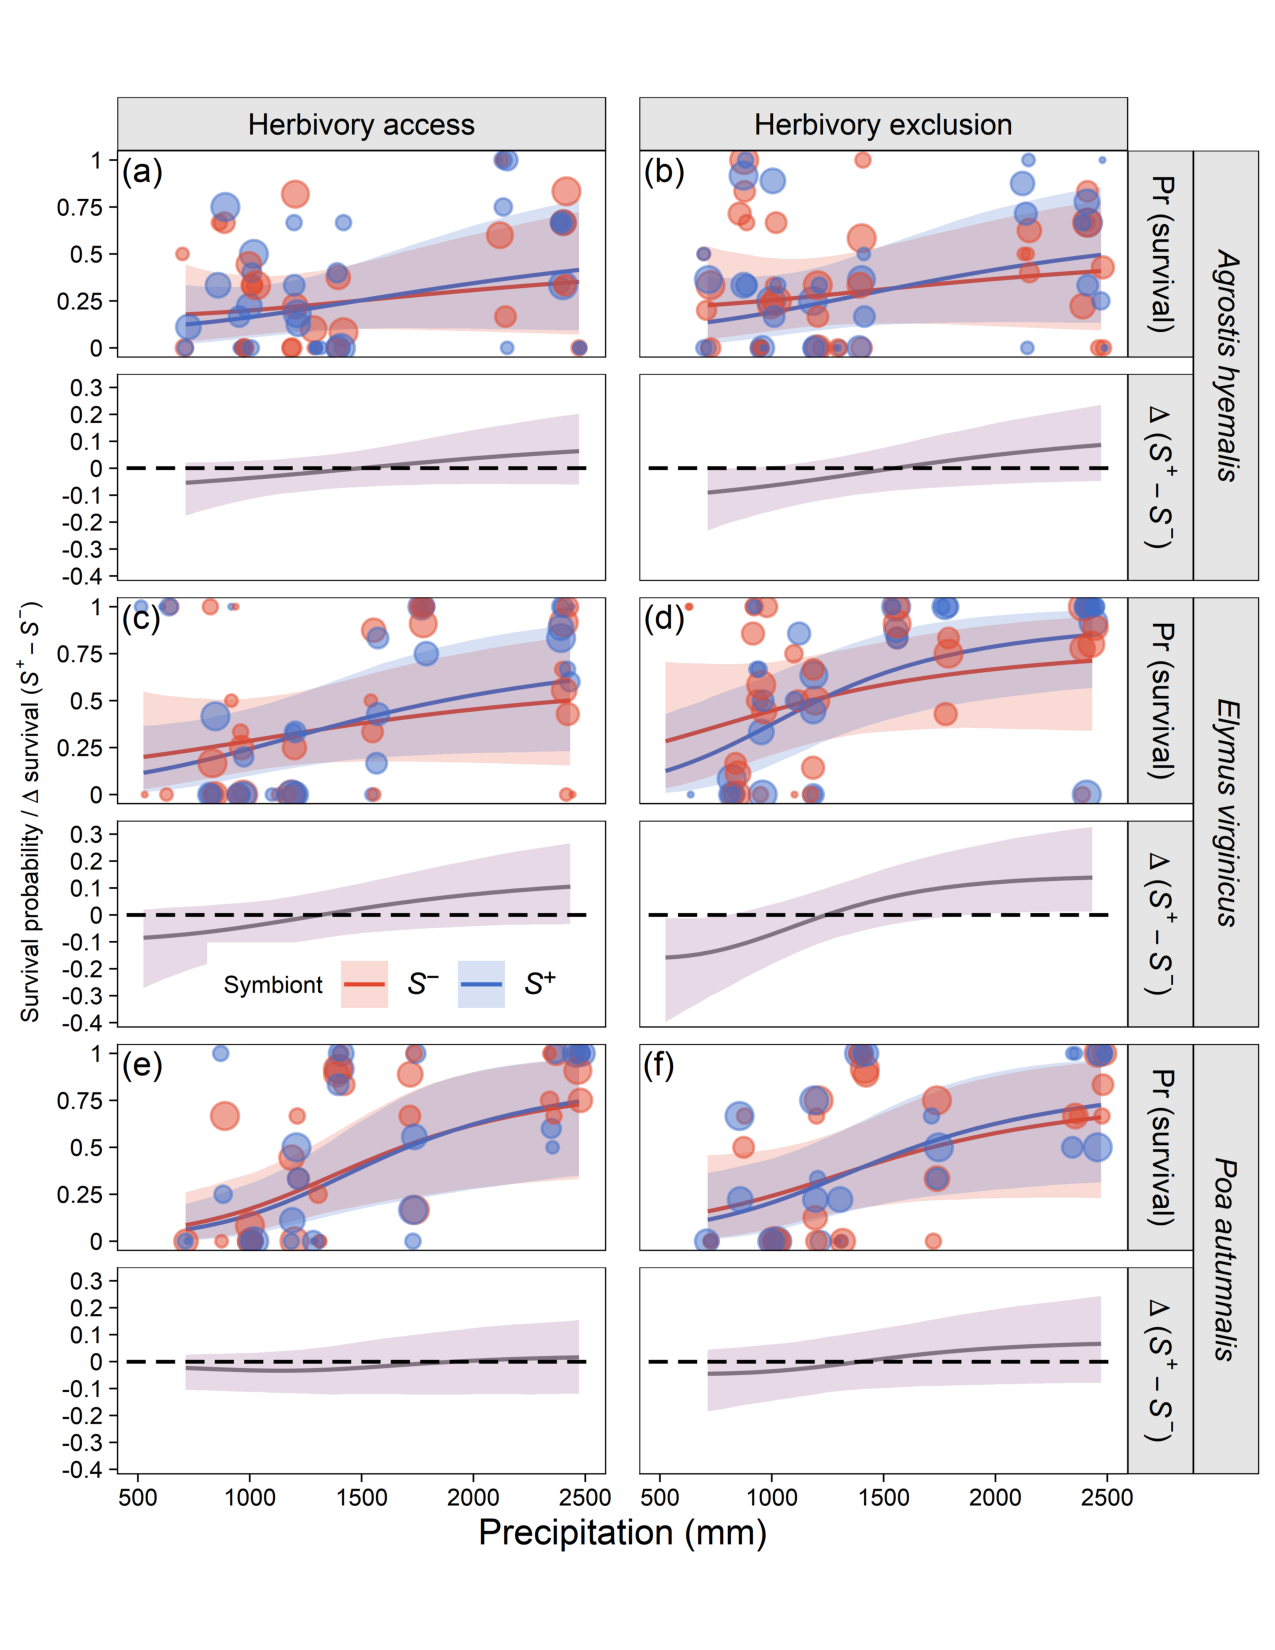
\includegraphics[width=\textwidth, trim=0 1.5cm 0 1cm, clip]{PrSurvival_diff.pdf}
\caption{Predicted survival probability (upper panels) and symbiont effect ($\Delta$ = $S^+ - S^-$; lower panels) across the precipitation gradient. 
Lines and shaded regions show posterior means and 90\% credible intervals, respectively. 
Points indicate observed plot means, with point size proportional to sample size.
Horizontal dashed line denotes $\Delta = 0$. 
Panels are arranged by species and herbivory treatment (herbivore access and exclusion).}
\label{fig:Surv}
\end{figure}

\clearpage

\captionsetup[figure]{list=no}
\begin{figure}[htbp]
\centering
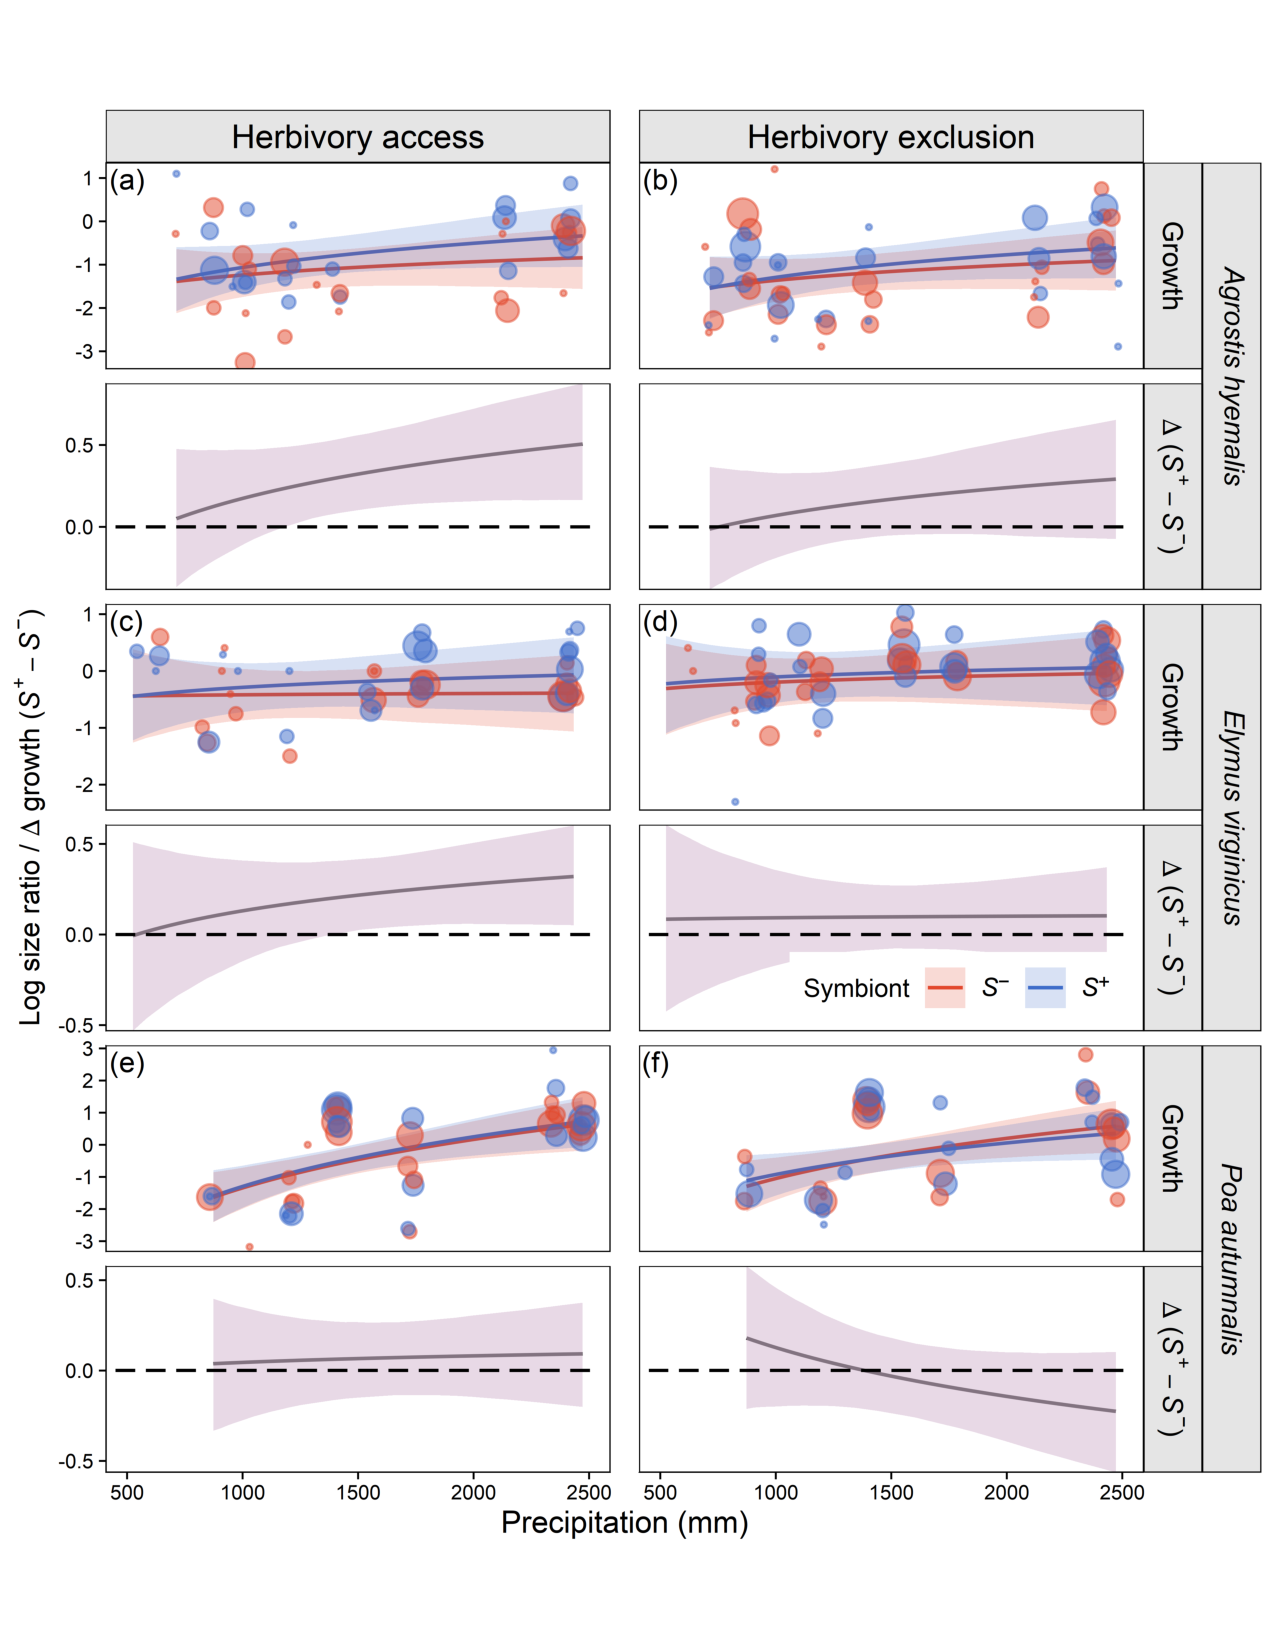
\includegraphics[width=\textwidth, trim=0 1.8cm 0 1.5cm, clip]{Growth_diff.pdf}
\caption{Predicted growth (log size ratio; upper panels) and symbiont effect ($\Delta$ = $S^+ - S^-$; lower panels) across the precipitation gradient. 
Lines and shaded regions show posterior means and 90\% credible intervals, respectively. 
Points indicate observed plot means, with point size proportional to sample size.
Horizontal dashed line denotes $\Delta = 0$. 
Curves reflect models fitted on log precipitation.
Panels are arranged by species and herbivory treatment (herbivore access and exclusion).}
\label{fig:growth}
\end{figure}
\clearpage

%\captionsetup[figure]{list=no}
%\begin{figure}[t]
%\centering
%\includegraphics[width=0.95\textwidth]{../Figure/Inflorescence_diff_v.pdf}
%\caption{Predicted inflorescence production (upper panels) and symbiont effect ($\Delta = S^{+} - S^{-}$; lower panels) across the precipitation gradient. 
%Lines show posterior means with 90\% credible intervals. 
%Points indicate observed values. 
%Horizontal dashed line denotes $\Delta = 0$. 
%Panels are arranged by species and herbivory treatment (herbivore access and exclusion). 
%All panels share a common x-axis for illustrative purposes; some species 
%extend beyond their observed precipitation range.}
%\label{fig:inflo}
%\end{figure}

\captionsetup[figure]{list=no}
\begin{figure}[htbp]
\centering
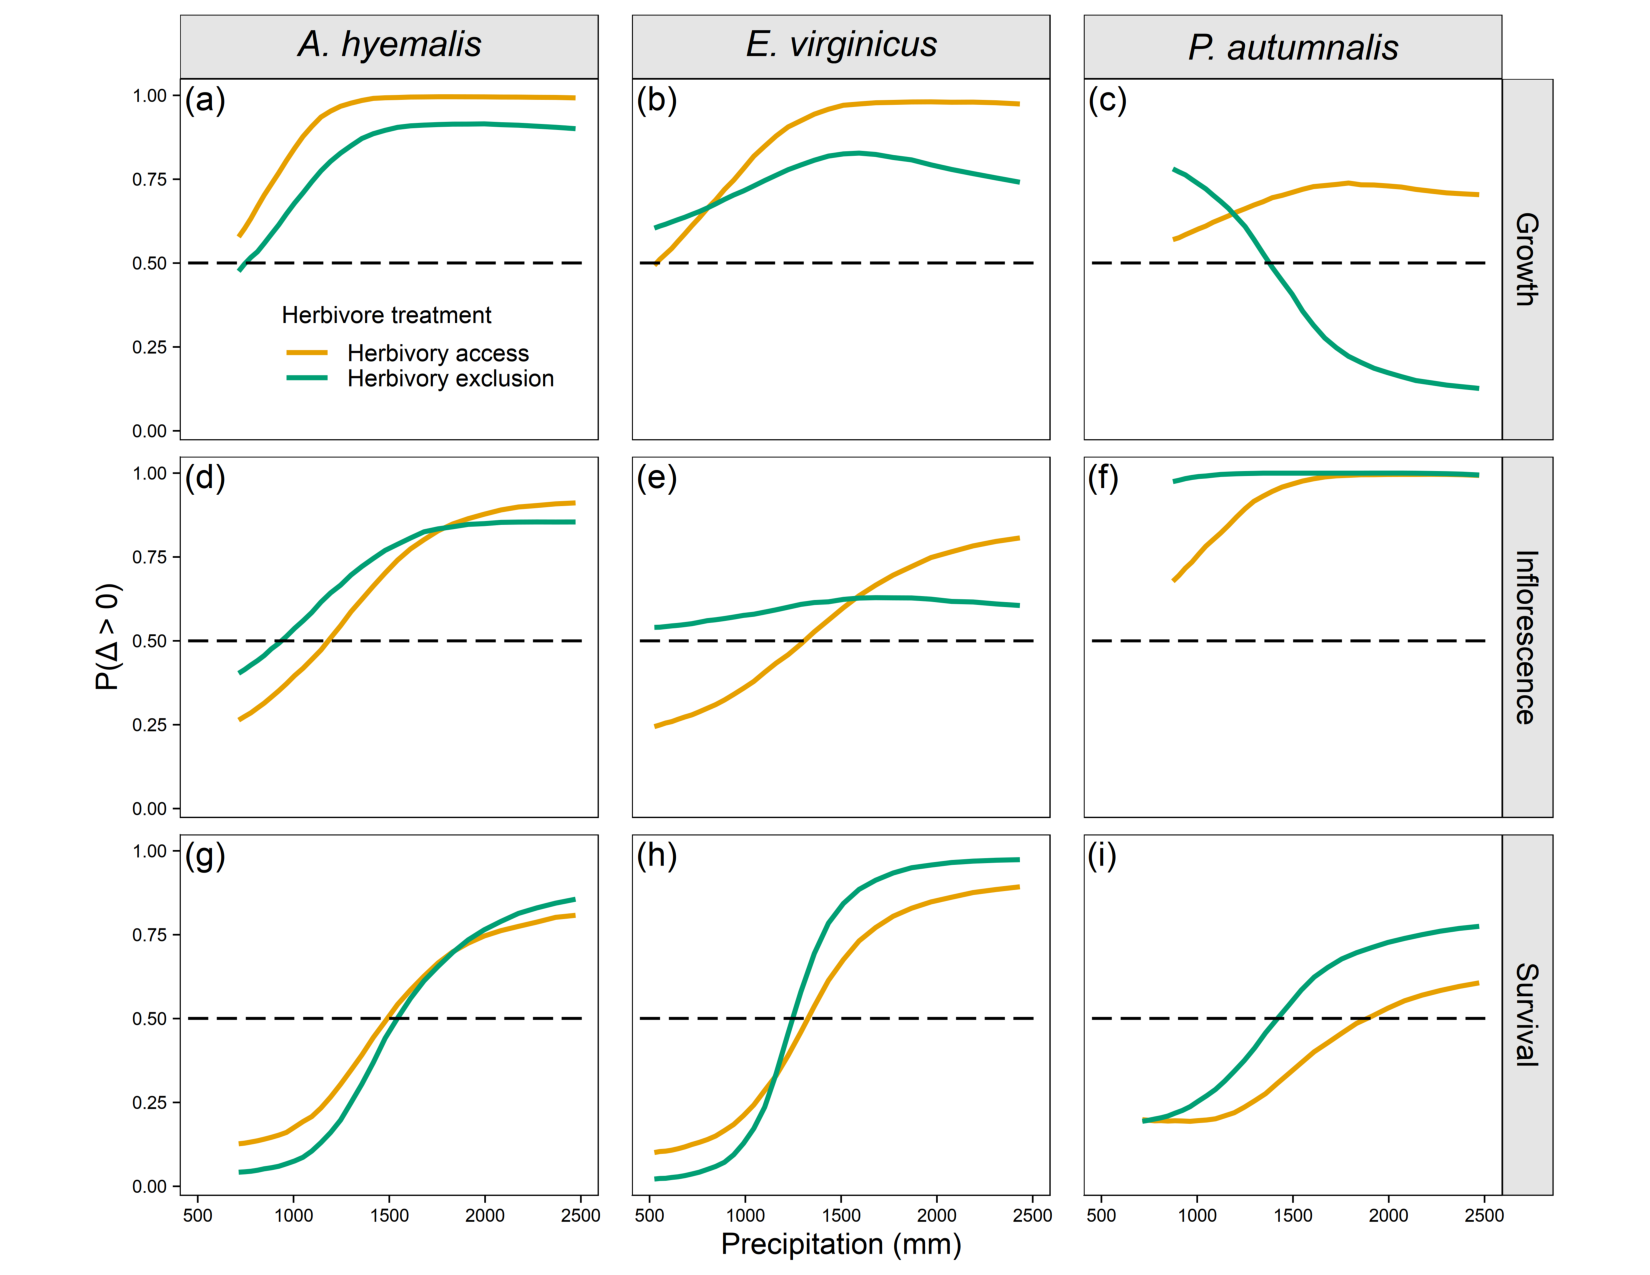
\includegraphics[width=1\textwidth]{All_traits_diff_stat_lower.pdf}
\caption{
Probabilities of positive endophyte effects on survival, growth, and inflorescence production across precipitation gradients and under herbivore access or exclusion for \textit{A. hyemalis}, \textit{E. virginicus}, and \textit{P. autumnalis}. Panels show the probability that the difference in vital rates between $S^+$ and $S^-$ hosts is positive ($\Pr[\Delta > 0]$). Values closer to 1.0 indicate high confidence in an $S^+$ advantage, values closer to 0.0 indicate high confidence in an $S^-$ advantage, and values close to 0.5 indicate no difference between $S^+$ and $S^-$. 
}
\label{fig:allstat}
\end{figure}
\clearpage

\captionsetup[figure]{list=no}
\begin{figure}[htbp]
\centering
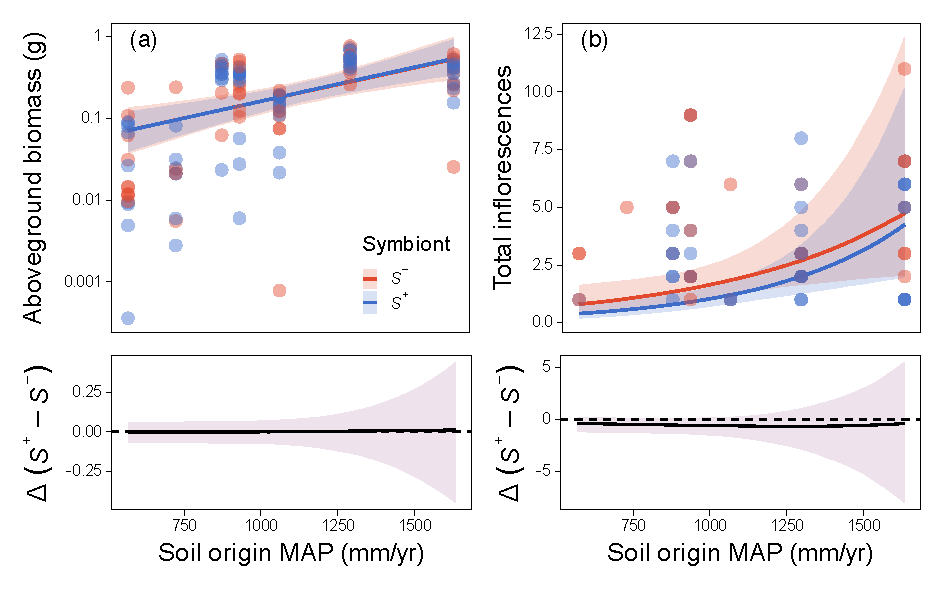
\includegraphics[width=0.9\textwidth]{Fig_Greenhouse_Combined.pdf}
\caption{Greenhouse experiment testing whether soil-origin precipitation modifies symbiont effects on host performance in \textit{Agrostis hyemalis}. Upper panels: posterior predictions for aboveground biomass (a) and total inflorescence production (b) across the 30-year mean annual precipitation of the soil-origin site (mm yr$^{-1}$), for symbiont-present ($S^+$) and symbiont-absent ($S^-$) plants; points are observed values, lines are posterior medians, and shaded ribbons are 95\% credible intervals. Biomass was modeled on the log scale and is shown on a logarithmic axis. Lower panels: posterior contrast between symbiont treatments ($\Delta = S^+ - S^-$) for the response shown above; the dashed line marks no difference between treatments.}
\label{fig:biomass_inflo}
\end{figure}
\clearpage

\end{document}